\chapter{Reference implementation of suggested framework\label{cha:chapter5}}

This chapter describes the concrete implementation of common aspects of the proposed framework as well as individual domain specific implementation. The in the concept, compare chapter \ref{cha:chapter4}, described introduction of libraries to enable an simple and adaptable solution is applied on the common aspects of the framework. The domain specific implementations provide an evidence about the generalization of the common elements as well as the applicability of the entire framework to specific domain. This chapter also discusses technologies as basis of the framework. 

\section{Environment and underlying frameworks\label{sec:env}}

\subsection{Technical container framework}

The use of the technical container framework promises the abstraction and simplification available data processing frameworks offer. Using such a framework contributes a stable environment as basis. Under the consideration of the outlined concept, especially the pipeline approach, the best fitting container framework is chosen from the family of stream processing frameworks. Stream processing enables a continuous delivery of prepared data, ships with features enabling processing guarantees.
\\\\
Consequently the following alternatives must be considered as container framework:
\begin{itemize}
\item Native stream processing engine of high level programming language
\item Distributed stream and data processing frameworks
\item Single node 3rd party stream processing frameworks\\
\end{itemize}

\noindent\textbf{Native stream processing engine of high level programming language:}

\noindent High level programming languages like Java already provide a library for processing data as a stream\cite{urma_2017}. They offer basic data processing functions like \textit{map(.)}, \textit{fold(.)} or \textit{filter(.)}. The barrier of applying a native stream processing framework is compared to external libraries relatively low as the nature of the language is preserved. Another benefit from using such a library are lower compatibility issues and fewer external dependencies. It is to favor to reduce maintenance overhead of software by reducing the number of external dependencies. 

The main drawback of internal processing engines is often that the connectivity to data sources and data sinks is limited. For example do Java streams only provide a connector to files in a local file system. If databases or message queues are plugged in custom stream sources need to be implemented. As the overall goal of the proposed framework is the unification of data across several sources native stream processing engines can not be considered in this concrete implementation.
\\\\
\textbf{Distributed stream and data processing frameworks:}

\noindent In section \ref{sec:containerframework} we already spoke about the trend of distributed data processing frameworks. Framework like Apache Flink, or Kafak Streams are specialized on data processing and provide a solid environment of features required for the proposed framework. Especially the aspect of distributed processing seems interesting when it comes to big amounts of data. Such framework minimize the implementation overhead due to distributed memory management and network communication. They also provide a broad set of connectors to different data sources and sinks. For example Apache Flink lists 13 connectors to 3rd party sources \cite{flink_streaming_2017}. 

A minor drawback is the dependency on external developers. Every externally introduced program code can, in the worst case, contain bugs. Restrictions regarding features are set by other developers and their overall focus and road map of the library or framework. A more significant disadvantage is that this frameworks are designed to run on a distributed, clustered system only. Some of the framework do in fact provide a local execution mode, but this is often only recommended for development purposes but not for production environment. Not only for the sake of simplicity also to minimize the the complexity of the system it is necessary to find a framework that allows single node deployment. It is also to mention, that throughput is not listed as a requirement for the feature extraction framework. It is also not to forget, that the frameworks concept is designed in such a ways, that it does not depend on the underlying data processing framework. Hence, if the requirement for distribution arises, the framework implementation can be ported.
\\\\

\textbf{Single node 3rd party stream processing frameworks:}

\noindent From the previous two paragraphs we learned, that a 3rd party stream processing engine is a desirable ways to go. The requirement for reducing implementation complexity of a showcase example brings the demand for single node deployment. Unfortunately the list of frameworks satisfying the restrictions above is short. The Akka framework for actors\footnote{A Actors model is a mathematical model enabling parallel and concurrent data processing.} \cite{akka_2017} enjoys a brought acceptance among developers. This framework provides a streaming framework on top of Akkas actor model. Akka streams \cite{akka_streams_2017} have a excellent support through the close relation to the Scala programming language as well as a wide community support\footnote{More than 400 contributors on www.github.com/akka/akka.}. Concerning the adaptivity of heterogeneous sources a community is established that provides connectors to more than 20 data sources, sinks, protocols and libraries. The Alpakka library \cite{alpakka_2016} contains among others connectors to the major database systems like MongoDB, Hbase or Cassandra, as well as to file formats as CSV, XML or text files. The repertoire of Alpakka connectors also lists transfer protocols like FTP, which can be beneficial for integrating remote sources of customers on a file basis.
\\\\
For the proof of concept implementation of the automation framework Akka streams is chosen as the container framework and extended by the Alpakka library. 

\subsection{Data transfer layer}
To maintain the concept of modularization and pluggability of the framework while using Akka streams it is essential to introduce a data transfer component. The data transfer layer is part of the assemble of technologies that build the container framework. Singular components realized in Akka streams need to be connected through that data transfer layer. This component is also used for the realization of the error pipeline as described in section \ref{sec:errorpipeline}. An easy to use candidate for such an application is Kafka. The streaming platform works with a publish-subscriber pattern and is a fault tolerant system for connecting software components. The ability to create streams, known as topics, comes beneficial for the error pipeline. Here each step can define its own topic to which faulty data can be published and distinguished afterwards.

\subsection{Programming language and libraries}
The choice of the target programming language primarily depends on the application use case. Data processing and data transformation are often non-side-effecting applications of functions on single information entities. This can be seen on the concept of UDFs in the proposed framework. The conclusion can be made, that a functional programming language is well suited for this thesis' implementation. 

A second, very related aspect, is the API of the underlying framework. As the underlying framework is chosen by the best fit for the thesis' use case it is natural to imply that the technical container frameworks language is the right fit. 

Scala as a functional programming language combines the two previous aspects. This brings us to the conclusion, that the Scala programming language is a perfect candidate for a example implementation of the framework and development of the demonstrative use case.

\subsection{Internal data format}
The use of the data transfer layer urges the use of an internal common data encoding format. This aspect is already described in section \ref{sec:overalldesign}. Apache Kafka does not restrict the usage of certain data formats. Due the wide usage and human readability JSON is considered as a suitable internal data format. This also enables manual inspection of information entities on quality assurance tasks. 

\section{Implementation of input adapter and raw formats}

The implementation of the input adapter on the frameworks library level boils down to three main classes. A data loader, a data sink and a third component to wire up the former classes. 

\subsection{Implementation of the loader component \label{ssec:loadercomponent}}

A source specific data loader is a sub-class of the abstract generic class \textit{AbstractLoader}, compare the class diagram in figure \ref{fig:importer-diagram}, and is meant to hide the actual encoding format of the data source as well as to transform a source element of type \textit{IN} to raw type \textit{OUT}. A \textit{AbstractLoader} requires the implementation of the data source, which is defined as a \textit{Source}-object in the Akka streams framework and can be taken from the previously name Alpakka library. The abstract function \textit{tryParseElement($\cdot$)} is a function sub for the actual UDF that enables the mapping of the source schema of type \textit{IN} to the raw schema of type \textit{OUT}. The function \textit{handleFailed($\cdot$)} is called before an faulty element is written to the corresponding message queue in Kafka and can be overwritten in the case the user wants to introduce custom error handling.

As a concrete example a MongoDB loader was implemented and provided to to framework library. This example utilizes the ReactiveMongo driver\footnote{www.reactivemongo.org/} which is used to implement the Akka stream source as the class \textit{AbstractLoader} requires.

\begin{figure}[htb]
  \centering
  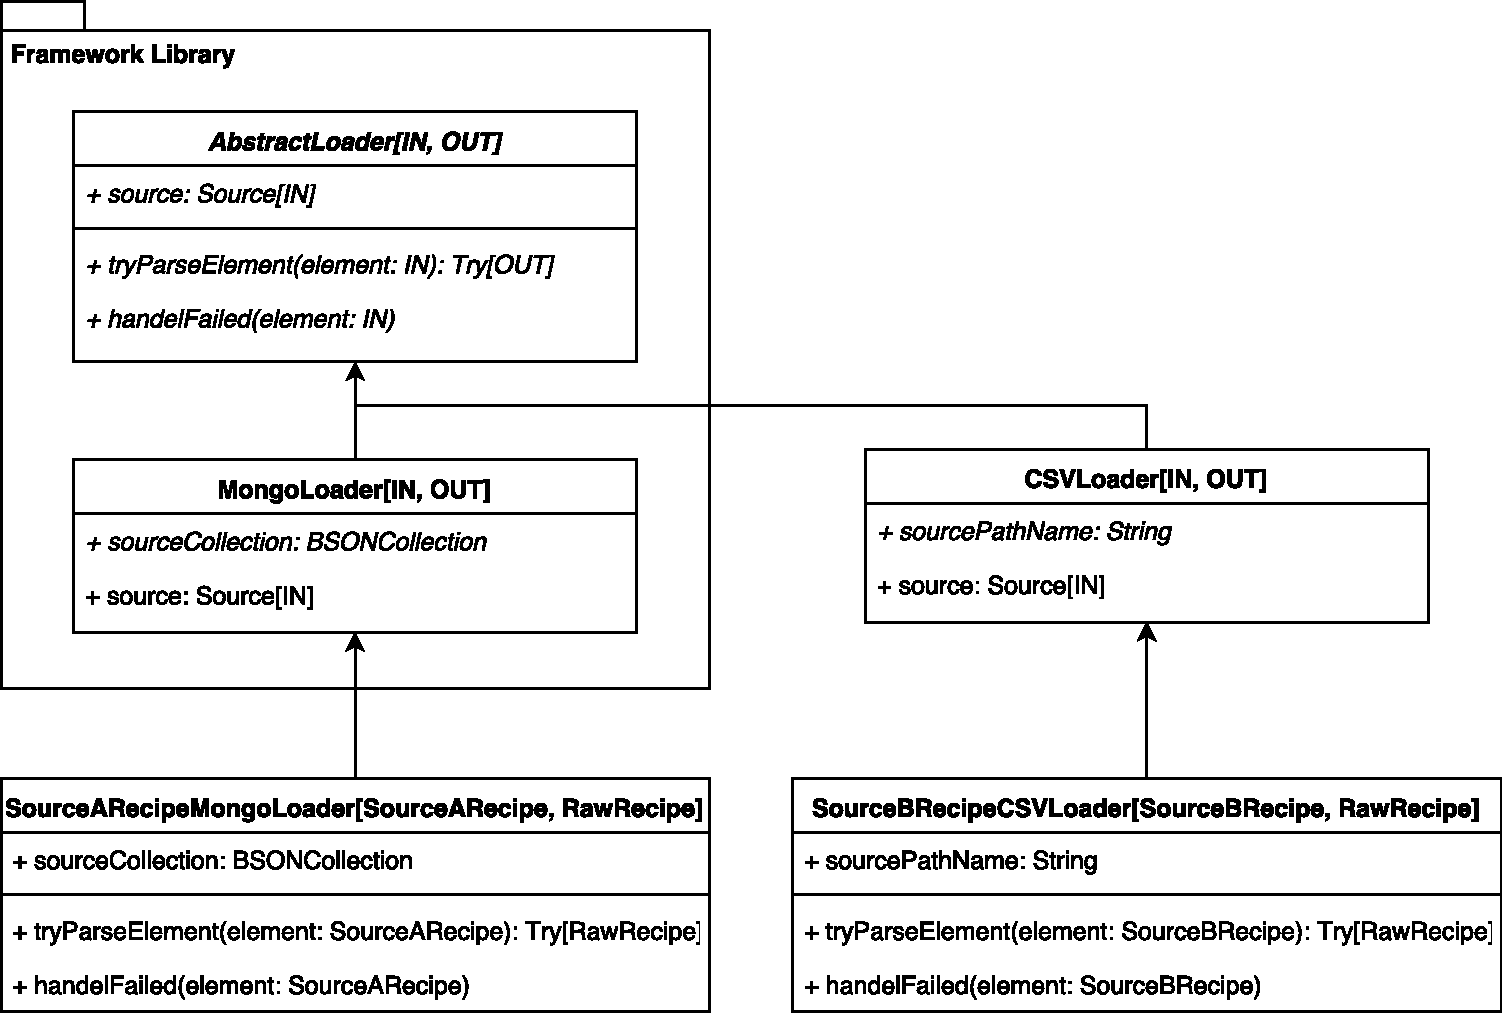
\includegraphics[width=0.9\textwidth]{importer-diagram}\\
  \caption{Class diagram of data loader library and implementation}
  \label{fig:importer-diagram}
\end{figure}

In the third level of the inheritance hierarchy the source and raw format needs to be specified. Here is also the implementation of the UDF located. The UDF takes a source specific element as parameter and must return a the defined raw entity. This is the only place where domain specific knowledge is introduced. This class is not part of the library.

\subsection{Definition and introduction of raw entities}
In the framework a raw entity is defined as global valid abstraction of information entities among all possible sources. To satisfy this specification it is necessary to declare redundant attributes for different sources. Taking a recipe as example, investigation on available data shows that for example ingredients are normalized into three levels:
\begin{itemize}
\item "amount unit name"
\item "amount unit", "name"
\item "amount", "unit", "name"
\end{itemize}
To find one raw format that satisfies the most possible sources, three different attributes are introduced in the raw recipe entity. This approach enables downstream processing steps to apply adequate rules for each of the three attributes and extract the highest level of normalization \textit{amount}, \textit{unit}, \textit{ingredient}. This level is desirable for post-preparation applications that use features build on amounts of ingredients or their names. It is also thinkable to simply choose the lowest level of normalization if the downstream application does not need detailed information. From this example we see, that the introduction of the abstract raw entity satisfies messy source data as well as reliability for downstream preparation steps. It perfectly fits the idea of a modularized software.

This core approach is not only applicable for recipes and their ingredients. It can be simply be transfered to other domains like product catalogs or person profile information.

\subsection{Implementation of the sink component for raw entities}

\begin{figure}[htb]
  \centering
  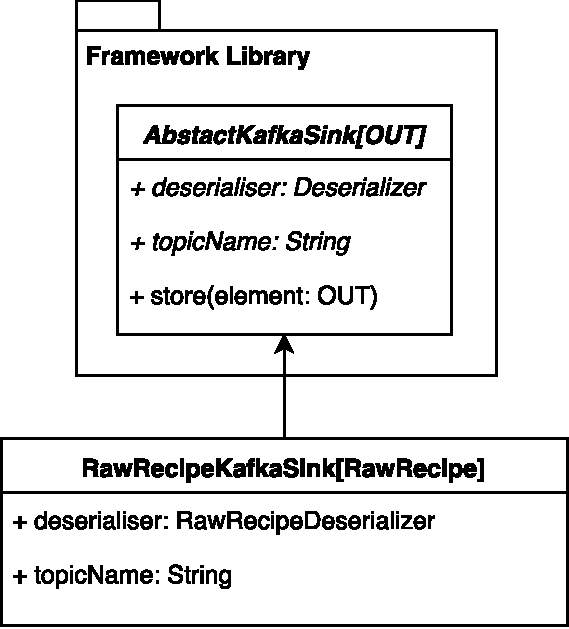
\includegraphics[width=0.3\textwidth]{importer-sink}\\
  \caption{Class diagram of input adapter sink and implementation}
  \label{fig:importer-sink}
\end{figure}

The second component from the input adapter is the sink to the underlying transportation layer. It is abstracted by the class \textit{AbstractKafkaSink}. The implementation must specify the serializer\footnote{A serializer is a software component, that defines how an specific class instance is created from a an different input format.} that is used to write the raw entity to the Kafka topic. Additional the topic name is to be provided. The class diagram in figure  \ref{fig:importer-sink} show the abstract implementation with the two mentioned attributes. Internally the publisher for the Kafka topic is defined in the function \textit{store(.)}.

\subsection{Implementation of the adapter component}

As a third component a object must be created that wires up the previous two components, this means to combine the data source, the UDF and the typed data sink as one entire processing pipeline. For this a executable object is created that inherits the class \textit{AbstractImporterAdapter}. The class diagram can be seen in figure \ref{fig:import-adapter}. The two discussed custom implementations must be provided.

\begin{figure}[htb]
  \centering
  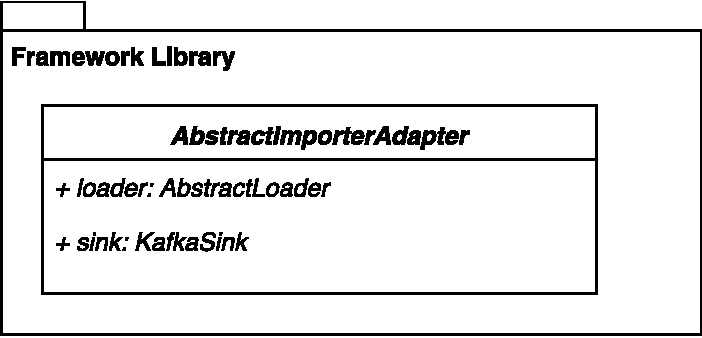
\includegraphics[width=0.4\textwidth]{import-adapter}\\
  \caption{Class diagram of input adapter sink and implementation}
  \label{fig:import-adapter}
\end{figure}

\subsection{Evaluation on library on recipe example}
The library for the import adapter is tested and showcased on the example of two sources of recipes. One source is a MongoDB collection\footnote{A collection in a MongoDB is equivalent to a table in a SQL database and contains a certain type of entities, called documents.}, the other source is a CSV file. Both sources contain recipes in a different schema. The input adapter library needs to be extend by a CSV loader. The extension is equal to the MongoDB source explained in section \ref{ssec:loadercomponent}, whereas the Alpakka source for CSV files is utilized. Concrete implementations of the both schemas as well s the raw recipe format are made and require very low programming work. The concrete implementation of the \textit{AbstractKafkaSink} only needs to provide a serializer for the global raw recipe. The utilization of the play-json\footnote{www.playframework.com/documentation/2.6.x/ScalaJson} library reduced the work to a minimum though a straight forward implementation of deserializers and serializers. The final importer job for both sources is a minimalistic implementation combining respectively the source and the common raw recipe Kafka sink.

\section{Implementation of the transformation pipeline}

The concept of the transformation pipeline suggests a component that can apply several transformation functions on raw entities of a deterministic schema and finally produces a generalized entity.

\subsection{Implementation of the common functionality}

The container framework Akka streams already provides a wide toolset of functionalities for data stream processing. As of the strong customization of transformation steps a less generic approach is chosen compared to the input adapters. 
\\\\
The main common component for the transformation pipeline are the input and output interfaces. Unifying the framework to one common data transportation layer and the concept of raw formats enables the reuse of components from the input adapter. Similar to the concept of the loader in the previous section a Kafka source is is implemented as part of the library for the transformation pipeline. The Kafka source is generic in that way that it is able to load any entity from a Kafka topic. The concrete implementation must then only provide a deserializer\footnote{A deserializer is a component, that defines how a class and its attributes are written to a specific output format.} for a concrete raw entity and the topic name.
\\\\
The component writing to the source, again Kafka, can be taken from the input adapter library classes. As outlined above, it is an generic implementation, that is able to write any object to a Kafka topic by providing a serializer and the topic name.

\subsection{Implementation of transformation pipeline steps}

Having the source and sink for the transformation pipeline provided by the library, the connecting transformation steps can be introduced. For the realization of the stepwise approach we take advantage of the board toolset of Akka streams. The concept in chapter \ref{cha:chapter4} already explains idea of UDFs and the usage for the transformation pipeline. Mainly two functions of Akka streams are necessary to build the required pipeline. Those are \textit{map(.)} and \textit{mapAsync(.)}. The implementation of the pipeline is based on a concatenation of those two function where each step takes the element to prepare, performs a transformation and finally returns an updated version of it. \textit{mapAsync(.)} has the additional benefit to call an external blocking resource without blocking the entire transformation pipeline. 
\\\\
A concrete implementation example that deals with raw recipe entities and transforms them to recipe entities is presented in the listening \ref{lst:pipeline}. It shows the transformation pipeline containing steps for preparation and parsing ingredients, instructions and image URLs. The source code of the individual functions is due to unimportance not listed here.

\begin{lstlisting}[style=myScalastyle,label={lst:pipeline},caption={Example transformation pipeline for raw recipes to recipes}]
val rawRecipeSource = KafkaRawRecipeSource("raw-recipes")
val recipeSink = KafakRecipeSink("recipes")

rawRecipeSource
  .map(ingredientService.processIngredients)
  .mapAsync(ingredientService.mapIngredients(_, 4, "de"))
  .map(processInstructions)
  .map(processServes)
  .map(createRecipe)
  .to(recipeSink)
\end{lstlisting}

\noindent The preparation and parsing steps in this concrete minimal example utilize the following technologies:
\\\\
\textbf{Regular expressions:}
The degree of automation of the feature extraction pipeline can be controlled by the effectiveness of applied transformation and parsing functions. Simple errors and deviations within the raw entity can be captured with regular expressions. Such a processing step is applied by calling \textit{ingredientService.processServes($\cdot$)}. It uses regular expressions that separate the field \textit{amount\_unit}. In this case a very deterministic input can be expected. Hence, a simple expression that matches on a combination of numbers and alphanumeric characters separated by zero or more spaces is sufficient. The capturing groups\footnote{A capturing group is a group of regular expressions that capture the text matched within that group as a unit.} for amount and unit enable a deterministic separation of both attributes for a given ingredient.
\\\\
\textbf{Self learning systems:}
As defined in the concept, the framework for feature extraction must also be able to learn from its input. This core requirement can easily applied in a further transformation function and the degree of learning defined by the implementing instance. An approach taken in the reference implementation for food recipes utilizes a full-text search engine and a continuous update of a learning data set for an increasing learning rate over time. 
\\\\
The implemented example of the framework uses Elasticsearch \cite{elasticsearch_2017} to overcome the varying manifestations of ingredient names in recipes. Elasticsearch is a search engine based on the Apache Lucene\footnote{www.lucene.apache.org/core/} project. The search engine supports full-text search on schema-free JSON documents powered by inverted indices\footnote{An inverted index is a lookup table where the alphabet of all possible words is listed and point to the documents in which they are contained.}. The idea is to find find the universal ingredient name by searching such with the raw ingredient string from the data source. A fuzzy\footnote{A fuzzy search on Elasticsearch finds all possible matches within a maximum edit distance.} search based on n-grams\footnote{A n-gram is a continuous sequence of substrings of length n of a underlying longer string (e.g. "reci", "ecip", "cipe" are all possible 4-grams for the string "recipe").} returns possible mappings of the raw ingredient string to universal ingredient names. 
\\\\
For example the string "Paprika, rot" will match the following universal ingredient names:
\begin{enumerate}
\item rote Paprika
\item Paprika
\item edelsüßes Paprikapulver
\end{enumerate}

This mapping can be taken and verified in a downstream quality assurance check. After a positive feedback the raw ingredient string (here "Paprika, rot") is stored with the ingredient Paprika as additional manifestation. Over time the data set contains several manifestations of one ingredient and enables better and more accurate mapping results. Over the long term the systems knowledge base is a list of ingredient documents containing the universal name and possible different wordings for each ingredient. The performance of the system is discussed in chapter \ref{cha:chapter6}.

\section{Implementation of output adapter}

The concept from section \ref{sec:componentsoutput} defines a component that provides the possibility of using several output formats. Figure \ref{fig:output-adapter} illustrates three different output adapters:
\begin{itemize}
\item Feature extractor
\item JSON serializer
\item Log appender
\end{itemize}

\begin{figure}[htb]
  \centering
  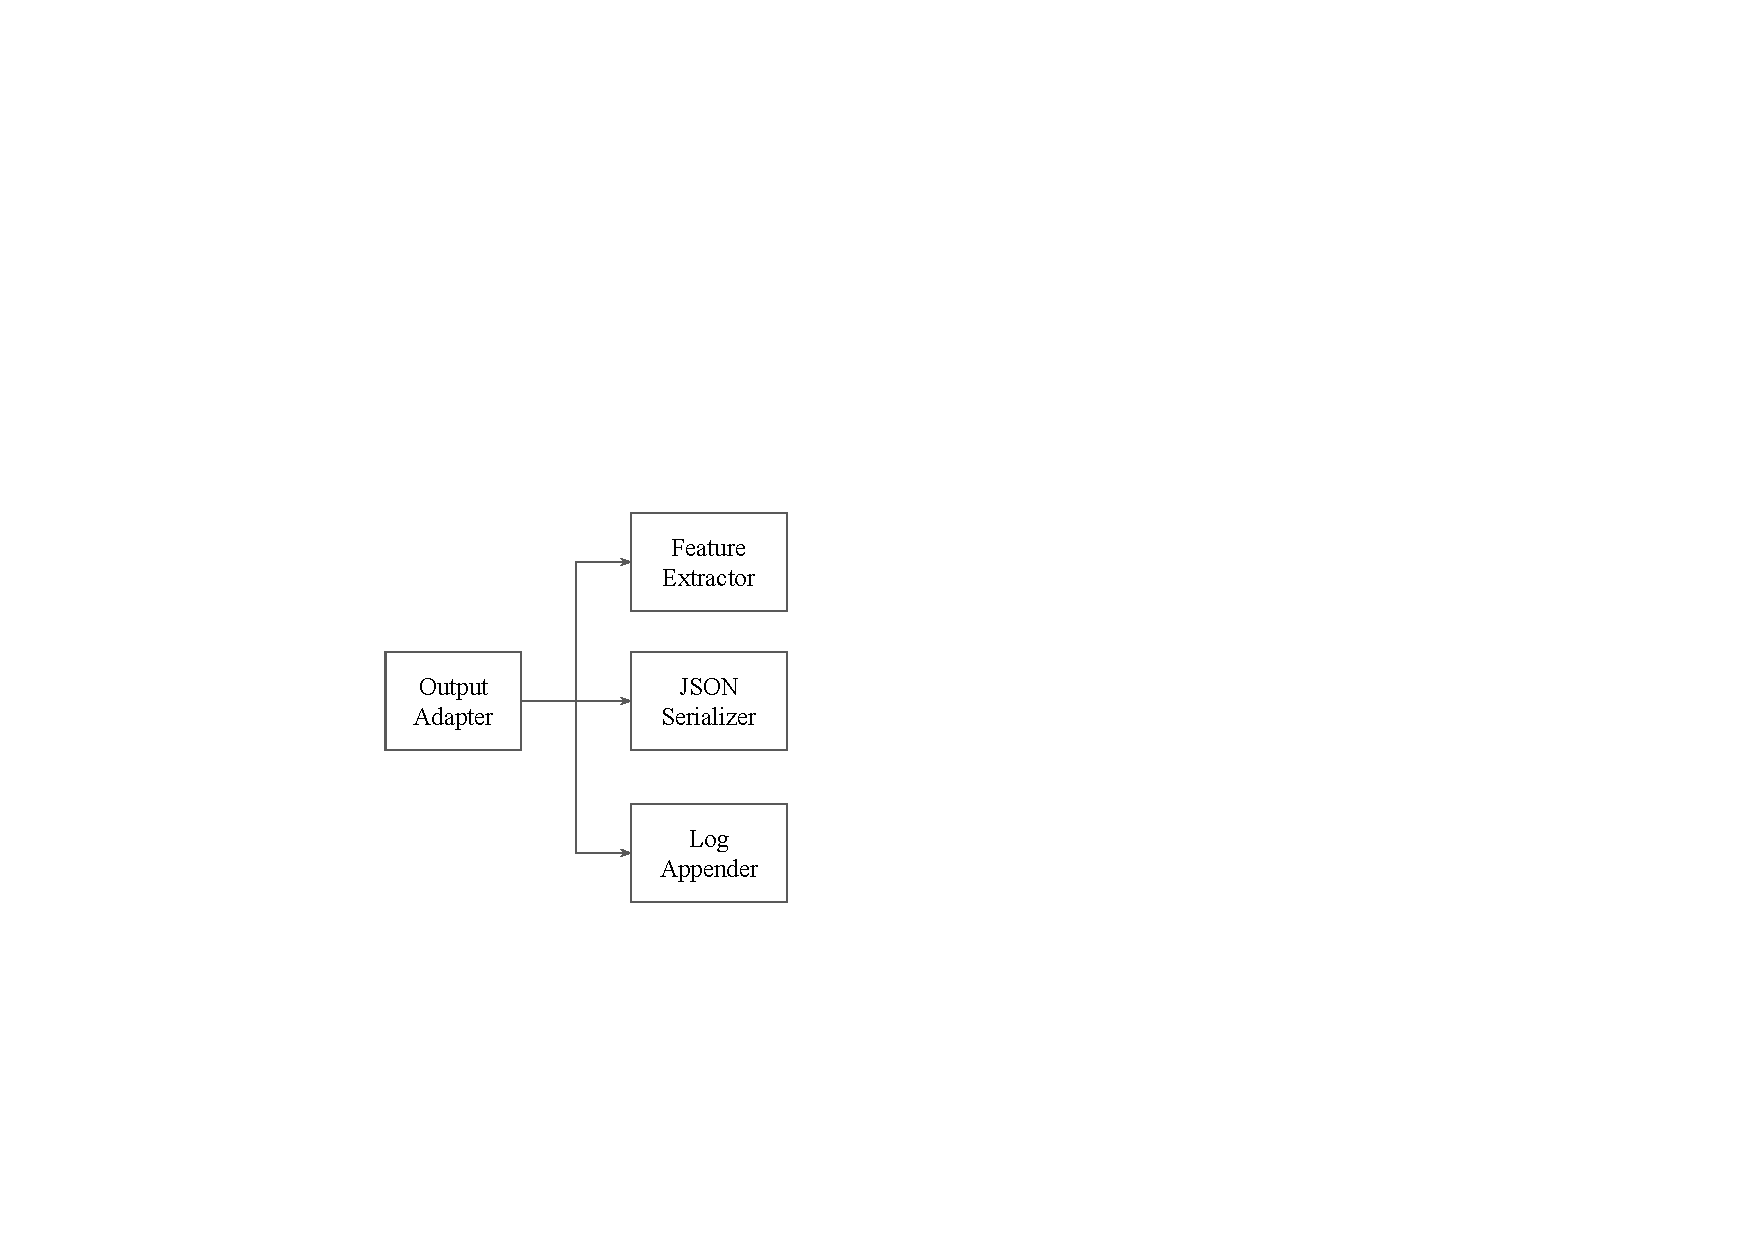
\includegraphics[width=0.4\textwidth]{output-adapter}\\
  \caption{Overview of message flow in the output adapter}
  \label{fig:output-adapter}
\end{figure}

The most important output adapter for a framework for automated feature extraction is clearly a feature extractor. The two further examples serve the visualization purpose. The in the proof of concept implemented JSON serializer adapter is used for deliver the homogenized data for a quality assurance fronted. The Log appender is used for streaming the processed data into a standardized logging system, such as Logstash\footnote{Logstash is processing pipeline for bundling logs. See www.elastic.co/products/logstash}. 
\\\\
The overall adaptability was achieved by the Akka streams API. With Akka streams data streams can be build, combined and spitted. For the output adapter the latter feature was used. Via simple DSL\footnote{Domain-specific language is a abstraction of a programming language for a specific domain} flow graphs of Akka streams can be set up. The listening \ref{lst:output} below shows a reference implementation splitting one input source stream into three outgoing steams. The DSL of Akka streams is very intuitive and perfectly suitable for such a use case. It causes low programming overhead and promises fast exchange and extension of the adapter component. The source is again a Akka stream source reading from the underlying transportation layer. \textit{RecipeKafkaSource} only has do define the deserializer for the specific entity and the Kafka topic name of recipes.

\begin{lstlisting}[style=myScalastyle,label={lst:output},caption={Example of akka streams graph DSL for splitting streams}]
val in = RecipeKafkaSource("recipes")

val adapter = builder.add(Broadcast[Recipe](3))

val featureExtractorSink = RecipeFeatureExtractorSink()
val jsonSink = JsonSink[Recipe]()
val logAppenderSink = LogAppenderSink[Recipe]()

in ~> adapter ~> featureExtractorSink
        adapter ~> jsonSink
        adapter ~> logAppenderSink
\end{lstlisting}

The \textit{RecipeFeatureExtractorSink} finally creates feature vectors from a cleaned and stable recipe information entity. It is up to the demand of the developer which features are extracted. As feature engineering is not part of this work, details are not discussed here. The literature provides several approaches and techniques about feature engineering \cite{mastering_feature_engineering_2017} \cite{liu_2001}. 
\\\\
For the reference implementation binary features of the recipe ingredients were extracted. A binary feature vector is a vector only containing zeros and ones. If a specific attribute is present in the entity to represent, the corresponding field is set to one, otherwise to zero. Here the ingredients are used as features. The unified ingredient names are hashed to determine the the index within the the feature vector. This approach is reliable, as first, the possible manifestations of universal ingredients is finite, and second, the used hashing algorithm, here murmur-hash, returns a deterministic hash for each possible string. To reduce sparsity of the resulting feature vector most common ingredients and most uncommon ingredients where removed. A TF-IDF was used to achieve this. The term frequency - inverse document frequency is used in feature extraction to find significant features. For reference see the above provided literature.

\begin{figure}[htb]
  \centering
  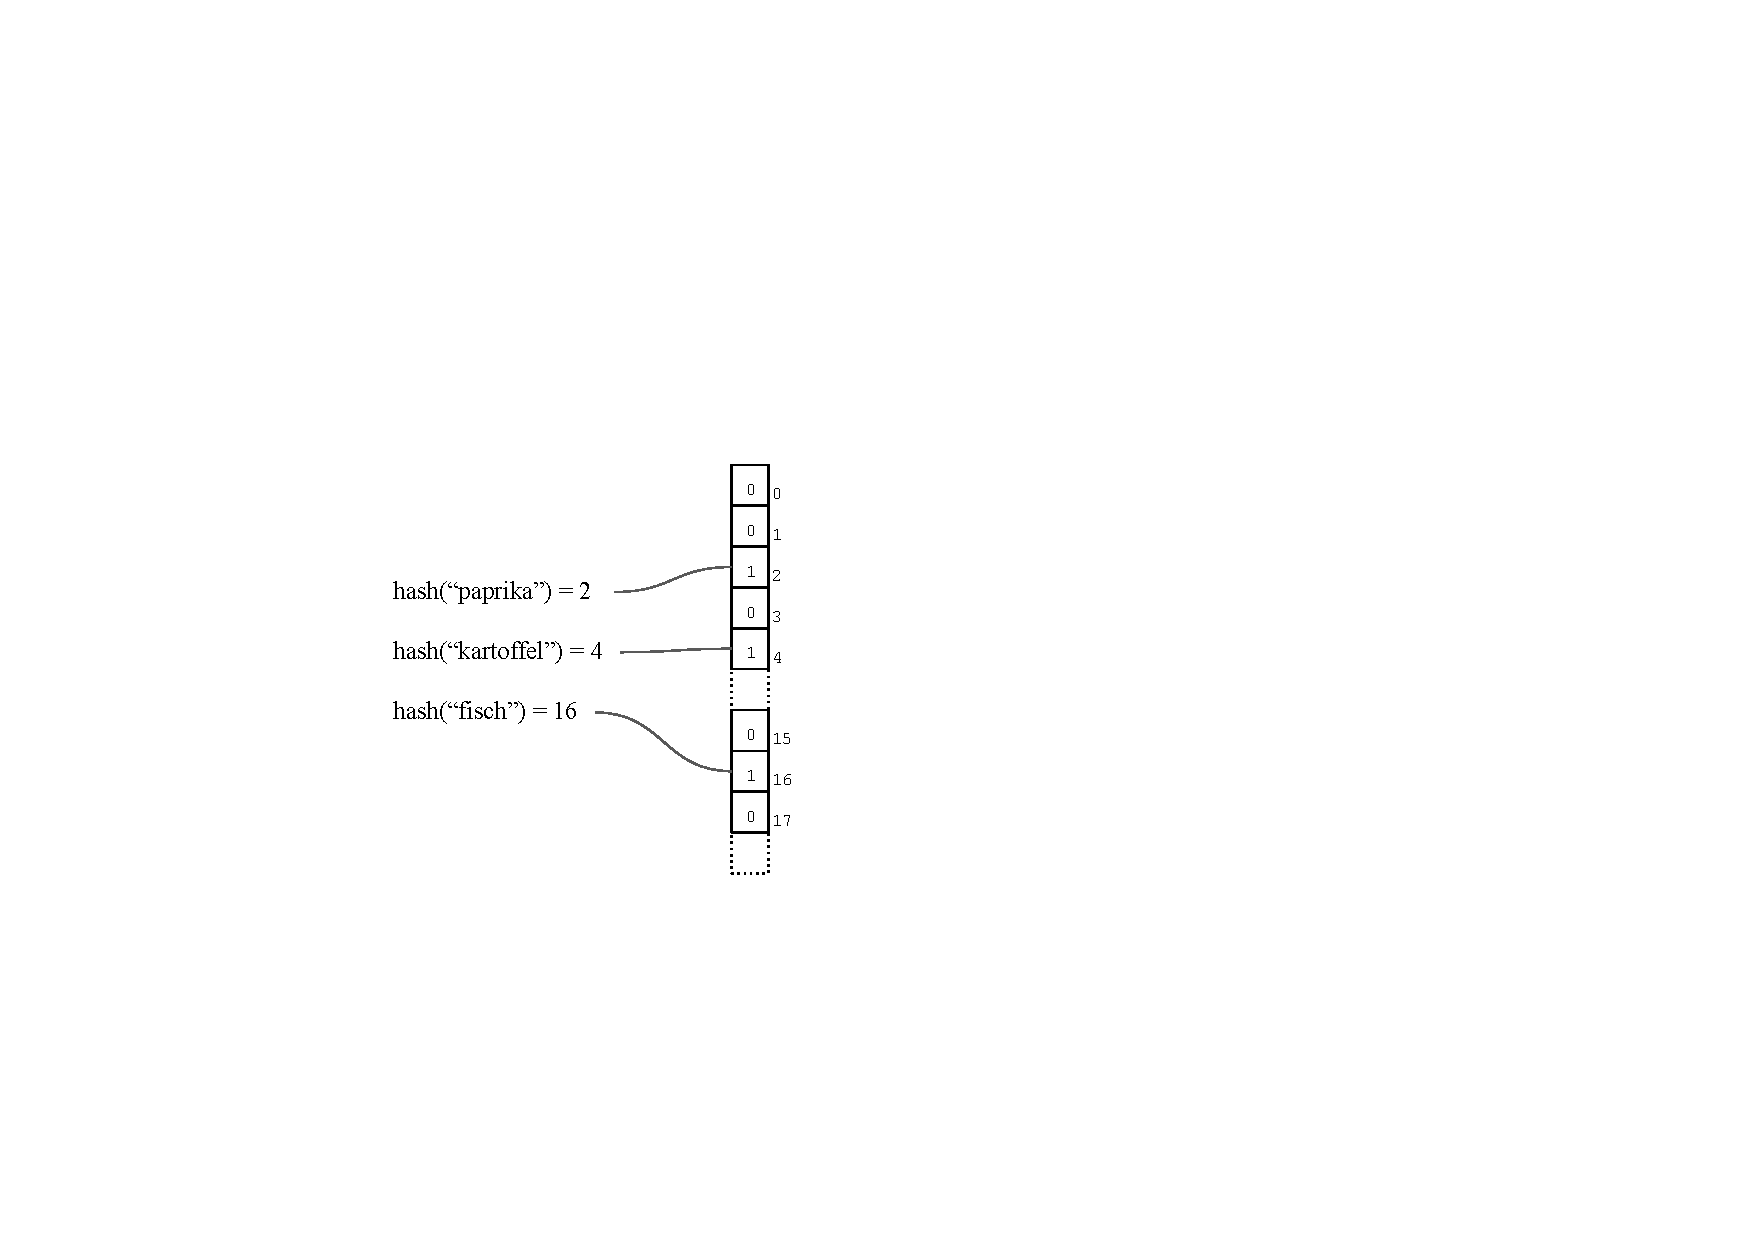
\includegraphics[width=0.4\textwidth]{bin-feature}\\
  \caption{Binary feature vector for the ingredients: paprika, kartoffel and fisch}
  \label{fig:bin-feature}
\end{figure}

\section{Implementation of a quality assurance and error handling interface}

The quality of the out coming data is critical. Several aspects about that are discussed in the previous chapters. From an implementation point of view, the quality assurance can be considered as further step in the transformation pipeline. To be more accurate the quality assurance step must be the finalizing step before the data are send to the output adapter and features are extracted.
As the implementation of an graphical user interface for quality assurance and administrative purposes is a very work and time costly project, only the data interface and the applicability within the suggested framework is given. 
In the concrete case, this means that particular data are run through the quality assurance step. Whether an entity needs to be checked or not can be determined automatically. For instance if the regular expression on the field \textit{serves} does not apply. As in the ingredient mapping step suggestions from the self learning system are given, in the concrete implementation every entity runs through a finalizing manual check. This can be reduced in future if learning system produces more reliable suggestions. 
The implementation for the quality interface sees a additional Kafka topic. After the transformation pipeline the entities are written to a dedicated quality assurance topic. The quality assurance application fetches the data from there, review is done and the entities are written back to new Kafka topic. From there the output adapter fetches the quality assured entities and features are extracted subsequently. The same principal is applicable for the error pipeline. The application can as well fetch data from those topics and re-introduce them into the topic for the generalized entities.

\section{Conclusion}

Concluding it can be said, that the choice of the underlying container framework Akka streams and Kafka as well as the programming language Scala plays well together with the domain of automated data preparation. The available libraries and the introduced custom library reduced the implementation overhead for a processing pipeline for unification of semi-structured data. The idea of an additional abstraction layer on top of the data transfer component, Kafka and the Akka streams, enables a simple adaption of the concrete framework implementation for different sources, entities and domains.
